% Solution: Tadelis (2013) Exercise 8.10 "Playing It Safe". Input by \solitem.
% Reused from lista-reais-lectures-01-04-solutions/item15.tex, deepened (expected-payoff table,
% interpretation, common mistakes). Check: check_B_L03.py.
\begin{exsol}{Tadelis Exercise 8.10}{172}{Exam}{3}
\asked Player~1 either plays safe ($S$, payoffs $(3,3)$) or risks ($R$) a simultaneous
$2\times2$ game with player~2. (a) Draw a tree and count its proper subgames; (b) say whether
other trees would do; (c) write the normal form; (d) find all Nash and subgame-perfect equilibria.

\method Extensive form with an information set for the simultaneous stage (Lecture~3,
slides~22--23; Tadelis \S7.1, Def.~7.2, p.~135); proper subgames (Lecture~4, slides~14--16;
Tadelis Def.~8.2, p.~154, which counts the whole game); strategies as complete plans (Lecture~3,
slide~25; Def.~7.4, p.~138); SPE by replacing the subgame with each of its Nash equilibria
(Lecture~4, slide~17; Tadelis \S8.2, Def.~8.3, p.~157; the voluntary battle of the sexes, Lecture~4,
slide~19, has the same structure). Mixed equilibria by the principle of indifference (Lecture~3,
slides~10--12; Tadelis \S6.1--6.2, pp.~101--114).

\solution
\textbf{Notation.} After $R$, player~1 chooses $C$ or $D$ and player~2 chooses $A$ or $B$
without seeing it. $p = \Pr_1(C)$, $q = \Pr_2(A)$ in the subgame.

\textbf{(a) Tree and subgames.}
\begin{center}
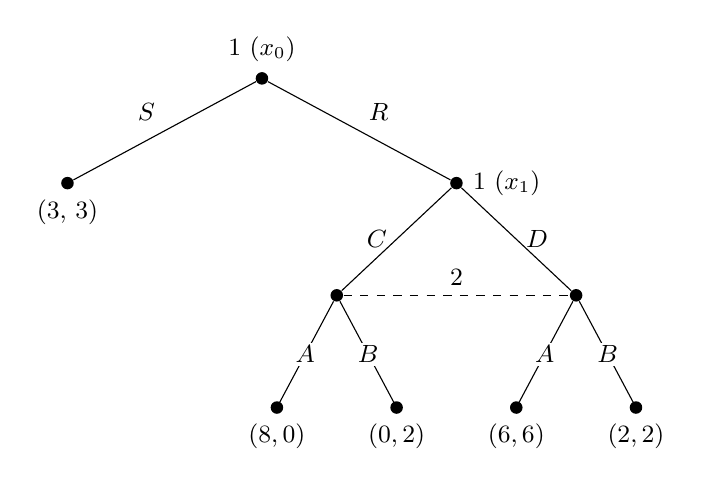
\begin{tikzpicture}[scale=0.95,dot/.style={circle,fill,inner sep=1.6pt},
  every node/.style={font=\small}]
  \node[dot,label=above:{1 ($x_0$)}] (r) at (0,0) {};
  \node[dot,label=below:{$(3,\,3)$}] (s) at (-2.6,-1.4) {};
  \node[dot,label=right:{1 ($x_1$)}] (x1) at (2.6,-1.4) {};
  \node[dot] (c) at (1.0,-2.9) {};
  \node[dot] (d) at (4.2,-2.9) {};
  \draw (r) -- node[above left] {$S$} (s);
  \draw (r) -- node[above right] {$R$} (x1);
  \draw (x1) -- node[left] {$C$} (c);
  \draw (x1) -- node[right] {$D$} (d);
  \draw[dashed] (c) -- node[above] {2} (d);
  \foreach \x/\p/\lab/\pay in {0.2/c/$A$/{$(8,0)$}, 1.8/c/$B$/{$(0,2)$},
                               3.4/d/$A$/{$(6,6)$}, 5.0/d/$B$/{$(2,2)$}} {
    \node[dot,label=below:{\pay}] at (\x,-4.4) {};
    \draw (\p) -- node[fill=white,inner sep=1pt] {\lab} (\x,-4.4);
  }
\end{tikzpicture}
\end{center}
Player~2's two nodes form one information set (dashed). Candidate roots of a proper subgame are
the singleton nodes $x_0$ and $x_1$; player~2's nodes fail (each would cut her information
set). So the game has \textbf{two proper subgames}: the whole game and the simultaneous game that
starts at $x_1$ (one, if, like Gibbons, one does not count the whole game).

\textbf{(b) Other trees.} Yes. (i) In the simultaneous stage, player~2 can be drawn as moving
first at $x_1$ with player~1's two nodes joined in an information set; the strategies, normal
form and subgames are unchanged. (ii) A different tree also represents the story: player~1
picks $S$, $RC$ or $RD$ at the root, and player~2 has one information set over the nodes after
$RC$ and $RD$. Its normal form is the same up to merging $SC$ and $SD$ (it is the
\emph{reduced} normal form), but it has only one proper subgame, the whole game, so subgame
perfection there has no bite: every Nash equilibrium is subgame perfect. The choice of tree matters
for SPE whenever it changes which subgames exist; tree~(i) and the drawing in (a) are the
faithful ones, since $R$ is a real decision taken before the stage game.

\textbf{(c) Normal form.} Player~1 has two information sets, so
$S_1 = \{SC, SD, RC, RD\}$ (first letter at $x_0$, second at $x_1$); $S_2 = \{A, B\}$:
\begin{center}
\begin{tabular}{r|c|c|}
\multicolumn{1}{r}{} & \multicolumn{1}{c}{$A$} & \multicolumn{1}{c}{$B$}\\ \cline{2-3}
$SC$ & $3,\ \br{3}$ & $\br{3},\ \br{3}$ \\ \cline{2-3}
$SD$ & $3,\ \br{3}$ & $\br{3},\ \br{3}$ \\ \cline{2-3}
$RC$ & $\br{8},\ 0$ & $0,\ \br{2}$ \\ \cline{2-3}
$RD$ & $6,\ \br{6}$ & $2,\ 2$ \\ \cline{2-3}
\end{tabular}
\end{center}

\textbf{(d) Equilibria.}

\emph{Step 1: the subgame at $x_1$.} Best replies: $BR_1(A) = C$ ($8 > 6$), $BR_1(B) = D$
($2 > 0$), $BR_2(C) = B$ ($2 > 0$), $BR_2(D) = A$ ($6 > 2$). They cycle, so there is no pure
equilibrium. Player~2 is indifferent when
\begin{equation}
  u_2(A) = 0\cdot p + 6(1-p) \;=\; 2p + 2(1-p) = u_2(B)
  \;\Rightarrow\; 6 - 6p = 2 \;\Rightarrow\; p = \tfrac23 , \label{eq:tadelis-8-10-p}
\end{equation}
and player~1 is indifferent when
\begin{equation}
  u_1(C) = 8q \;=\; 6q + 2(1-q) = u_1(D)
  \;\Rightarrow\; 8q = 2 + 4q \;\Rightarrow\; q = \tfrac12 . \label{eq:tadelis-8-10-q}
\end{equation}
The unique equilibrium of the subgame is $(p,q) = (\frac23, \frac12)$, with values
\[
  u_1 = 8\left(\tfrac12\right) = 4, \qquad u_2 = 6\left(1 - \tfrac23\right) = 2 .
\]

\emph{Step 2: subgame-perfect equilibrium.} Replace $x_1$ by $(4,2)$. At $x_0$, $R$ gives $4 > 3$,
so player~1 risks. Since the subgame has a unique equilibrium, the SPE is unique:
\[
  \sigma^{\text{SPE}}:\ \text{player 1 plays } R \text{ and then } C \text{ w.p. } \tfrac23;\
  \text{player 2 plays } A \text{ w.p. } \tfrac12,\qquad \text{payoffs } (4, 2).
\]
In the normal form this is player~1 mixing $\frac23 RC + \frac13 RD$ against $\frac12 A + \frac12 B$.
There is \emph{no} pure-strategy SPE.

\emph{Step 3: all Nash equilibria.} Expected payoffs against $q$:
\begin{center}
\begin{tabular}{lcc}
\toprule
Player~1's strategy & $u_1$ given $q$ & player~2's gain $u_2(A) - u_2(B)$ against it \\
\midrule
$SC$, $SD$ & $3$ & $0$ \\
$RC$ & $8q$ & $0 - 2 = -2$ \\
$RD$ & $6q + 2(1-q) = 2 + 4q$ & $6 - 2 = +4$ \\
\bottomrule
\end{tabular}
\end{center}
\begin{itemize}
  \item $q \le \frac14$: $3 \ge 2 + 4q$ and $3 > 8q$, so $S$ is a best reply (strictly, for $q<\frac14$).
  With player~1 on $\{SC,SD\}$ in any mix, player~2 is indifferent, so any such $q$ is a best reply.
  \emph{Nash equilibria.} (At $q = \frac14$, $RD$ also ties at 3, but any weight on it would make
  $A$ strictly better, forcing $q = 1$; so player~1 stays on $S$.)
  \item $\frac14 < q < \frac12$: $RD$ is the unique best reply ($2+4q > 3$ and $2 + 4q > 8q$);
  then player~2 strictly prefers $A$, i.e.\ $q = 1$. Contradiction.
  \item $q = \frac12$: $RC$ and $RD$ tie at $4 > 3$; player~2 is indifferent only if
  $-2\Pr(RC) + 4\Pr(RD) = 0$, i.e.\ $\frac23 RC + \frac13 RD$. \emph{The SPE above.}
  \item $q > \frac12$: $RC$ is the unique best reply; then player~2 plays $B$, $q = 0$. Contradiction.
\end{itemize}
So the Nash equilibria are
\[
  \bigl\{\,(\text{any mix of } SC, SD;\ q) : 0 \le q \le \tfrac14 \,\bigr\}
  \ \cup\ \bigl\{\,(\tfrac23 RC + \tfrac13 RD;\ q = \tfrac12)\,\bigr\},
\]
and the \emph{pure} Nash equilibria are $(SC, B)$ and $(SD, B)$, both with payoffs $(3,3)$.
None of the first family is subgame perfect: each asks player~2 to play $A$ with probability at
most $\frac14$ in a subgame whose only equilibrium has $q = \frac12$. The ``threat'' to play $B$
deters $R$, but it is not credible once $R$ has been played.

\interp Playing safe is supported only by player~2's threat to play $B$ in the risky game. Once
the risky game starts, both must play its (mixed) equilibrium, which gives player~1 an expected
4, more than the safe 3, so he takes the risk. Player~2 is worse off ($2 < 3$): she would like to
commit to $B$, but cannot; a public, costly commitment (Lecture~4, slide~11: observable, sunk
moves) would be her only way to keep player~1 on the safe path. The exercise also shows that
subgame perfection can select a \emph{mixed} continuation, so the credibility test applies to
probabilities, not only to pure threats.

\verify \texttt{check\_B\_L03.py} confirms that the subgame has no pure equilibrium, solves
\eqref{eq:tadelis-8-10-p}--\eqref{eq:tadelis-8-10-q} with sympy, finds the pure Nash equilibria
$(SC,B)$, $(SD,B)$ of the $4\times2$ matrix, and scans $q$ over a grid of 241 points plus the
critical values $\frac14, \frac38, \frac12$: a Nash equilibrium exists exactly at $q \in
[0, \frac14]$ and $q = \frac12$, and at $q=\frac12$ the mix $(\frac23, \frac13)$ on $(RC, RD)$
passes the exact Nash test while $(\frac12, \frac12)$ fails. Output line: \texttt{tadelis-8-10:
unique SPE (R; 2/3 C; 1/2 A), payoffs (4, 2)}. Tadelis prints no answer.

\mistakes
\begin{itemize}
  \item Looking for a pure SPE: the subgame has none, so the SPE must use its mixed equilibrium.
  \item Swapping the indifference conditions: $p$ (player~1's mix) is pinned down by
  \emph{player~2's} indifference, and vice versa.
  \item Counting a subgame at each of player~2's nodes, or forgetting that $(SC, B)$ and $(SD, B)$
  are two distinct Nash equilibria.
\end{itemize}

\answer{(a) Tree above; two proper subgames (the whole game and the simultaneous game after $R$).
(b) Yes: player~2 can be drawn first in the stage game; a tree with root choices
$\{S, RC, RD\}$ gives the same reduced normal form but no proper subgame other than the whole game.
(c) Matrix above, $S_1 = \{SC,SD,RC,RD\}$. (d) Pure Nash: $(SC,B)$, $(SD,B)$; all Nash: player~1
on $S$ (any mix of $SC$, $SD$) with $\Pr(A) \le \frac14$, plus $(\frac23 RC + \frac13 RD,\ \frac12 A
+ \frac12 B)$. Unique SPE: $R$, then $C$ w.p.\ $\frac23$; $A$ w.p.\ $\frac12$; payoffs $(4,2)$. No
pure SPE.}
\end{exsol}
